\documentclass[12pt,letterpaper]{article}
\usepackage[utf8]{inputenc}
\usepackage[english]{babel}
\usepackage{amsmath, amsfonts, amssymb}
\usepackage{graphicx, lmodern, float, hyperref}
\usepackage{multirow, multicol, dcolumn, tabularx, array}
\usepackage[table]{xcolor}
\usepackage[none]{hyphenat}
\usepackage{fancyhdr} % lets you customize header and footer
\usepackage[nottoc, notlot, notlof]{tocbibind} % to use table of contents
\usepackage[left=2cm,right=2cm,top=2cm,bottom=2cm]{geometry}
 
 
\setlength{\parindent}{0em}
\setlength{\parskip}{1em}

\pagestyle{empty}

\pagestyle{fancy}
\fancyhead{} % to clear the default header and footer
\fancyfoot{}


% Changing header
\fancyhead[L] { \slshape \MakeUppercase{ECG 701 Microeconomics Homework}}
\fancyhead[R] { \slshape Chowdhury Amir Abdullah}

\fancyfoot[C] {\thepage}


\usepackage{tikz,pgfplots}
\pgfplotsset{width=10cm,compat=1.12}
\usepgfplotslibrary{fillbetween}
\usetikzlibrary{patterns}


% To include PDF
\usepackage{pdfpages}

% To include all the pages in the PDF file:
% \includepdf[pages=-]{myfile.pdf}

% To include just the first page of a PDF:
% \includepdf[pages={1}]{myfile.pdf}


\title{pgfplots}
\author{Chowdhury Amir Abdullah}
\date{\today}




\begin{document}

\maketitle


\begin{tikzpicture}
\begin{axis}[xlabel=x,ylabel=y]
\addplot[smooth] {{-x^2}};
\end{axis}
\end{tikzpicture}


\begin{tikzpicture}
\begin{axis}[
    axis lines = left,
    xlabel = \( Q \),
    ylabel = {\( P \)},
]



\addplot [
    domain=0:10,
    %samples=100,
    color=red,
]
{2};
\addlegendentry{\( P=2  \)}

\addplot[
	domain=0:5,
	thick,
	blue,
	dashdotted,
	->
]
{2};

\addplot [
    domain=0:10,
    %samples=100,
    color=blue,
    ]
    {-x+10};
\addlegendentry{\(  P=10-Q \)}

\end{axis}
\end{tikzpicture}







First example is 2D and 3D math expressions plotted side-by-side.

%Here begins the 2D plot
\begin{tikzpicture}
\begin{axis}
\addplot[color=red]{exp(x)};
\end{axis}
\end{tikzpicture}
%Here ends the 2D plot
\hskip 5pt
%Here begins the 3D plot
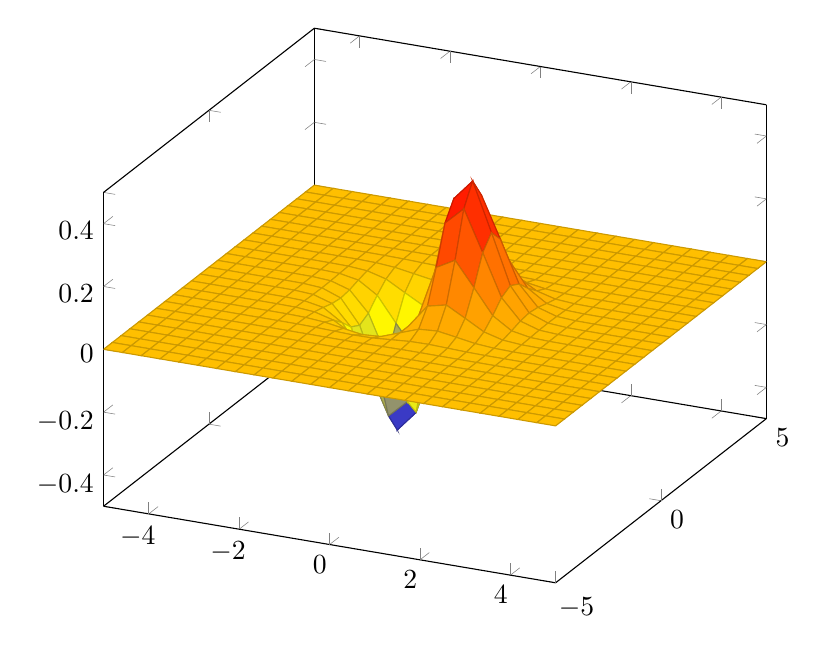
\begin{tikzpicture}
\begin{axis}
\addplot3[
    surf,
]
{exp(-x^2-y^2)*x};
\end{axis}
\end{tikzpicture}
%Here ends the 3D plot




\begin{tikzpicture}
\begin{axis}
\addplot[color=red]{-x+10};
\end{axis}
\end{tikzpicture}





\begin{figure}[h]
  \centering
  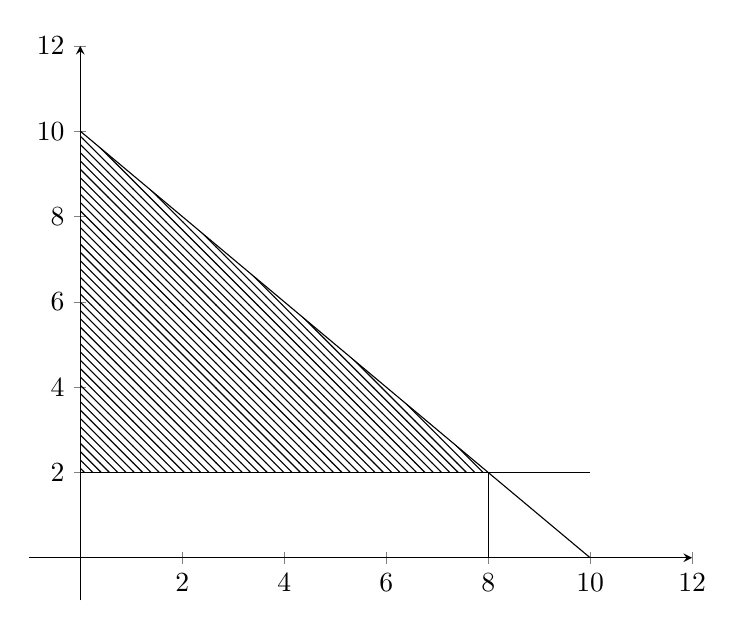
\begin{tikzpicture}
    \begin{axis}[
        xmin=-1, xmax=12,
        ymin=-1, ymax=12,
        axis lines=middle,
      ]
      \addplot[domain=0:10, name path=A] {-x+10};
      \addplot[domain=0:10, name path=B] {2};
      \path[name path=xaxis] (\pgfkeysvalueof{/pgfplots/xmin}, 0) -- (\pgfkeysvalueof{/pgfplots/xmax},0);
      \addplot[gray, pattern=north west lines] fill between[of=A and B, soft clip={domain=0:8}];
      %\addplot[gray, pattern=north west lines] fill between[of=B and xaxis, soft clip={domain=0:1}];
      %\addplot[gray, pattern=north west lines] fill between[of=A and xaxis, soft clip={domain=1:3}];
      \addplot +[mark=none] coordinates {(8, 0) (8, 2)};
    \end{axis}
  \end{tikzpicture}
\end{figure}


\end{document}
